\LevelOneTitle{相似原理}

\LevelTwoTitle{*力学相似}

\begin{definition}[力学相似]
	模型流动与原型(实物)流动在各对应空间点和对应时刻,对应物理量各自成一定的比例关系,包含:几何相似、运动相似和动力相似。
\end{definition}

三者的关系是:

\begin{figure}[H]
	\centering
	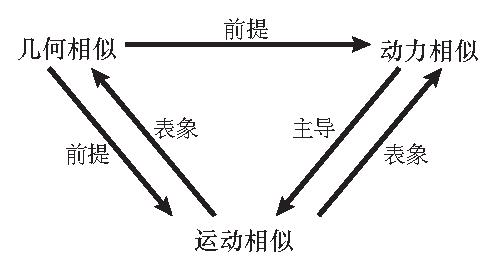
\includegraphics[scale=0.65]{figures/三种相似.eps}
	\caption{三种相似之间的关系}
\end{figure}

\LevelTwoTitle{准则数(2021·简答)}

\begin{enumerate}
	\item 雷诺数,惯性力与粘性力之比,适用于粘性流动,例如完全充满的管道内流动,数学表达为
	\begin{equation}
		Re = \dfrac{\rho V L}{\mu}
	\end{equation}
    \item 弗劳德数,惯性力和重力之比,适用于含有自由面的流动,例如明渠流、船舶形成的波运动,数学表达为
    \begin{equation}
    	Fr = \dfrac{V}{\sqrt{gL}}
    \end{equation}
    \item 欧拉数,压力与惯性力之比,适用于压力对流速分布影响较大的流动,例如空化效应,数学表达为
    \begin{equation}
    	Eu = \dfrac{\Delta p}{\rho V^2}
    \end{equation}
    \item 马赫数,惯性力和弹性力之比,适用于可压缩高速流动,例如加速喷管,数学表达为
    \begin{equation}
    	Ma = \dfrac{v}{a}
    \end{equation}
\end{enumerate}

需要掌握这四个准则数,韦伯数$We$和斯特劳哈尔数$Sr$了解即可。

\LevelTwoTitle{*近似模型法}

\LevelThreeTitle{什么是近似模型法}

\begin{definition}[近似模型法]
	保证模型流动和实物流动部分相似的方法,所谓“部分相似”,是指起主要作用的准则数相等。
\end{definition}

\LevelThreeTitle{雷诺相似}

适用于管道流动、物体绕流等,要求是:无自由面,重力对流态无影响,流速不高,可视作不可压缩流动,只考虑粘性力和压力,特征速度不能太大(太大将会影响压缩性)

\LevelThreeTitle{弗劳德相似}

适用于明渠流、船舶运动等,要求是:尺度不能太小,忽略表面张力,可视作不可压缩流动,粘性影响可以忽略或处于自模化状态,特征长度不能太小(太小将会影响粘性)

\LevelThreeTitle{什么是自模化}

\begin{definition}[自模化]
	流动相似本来取决于某准则数相等,但当其大到或小到一定程度时,即使准则数不等,流动也是相似的,这种状态就叫自模化。
\end{definition}